\chapter{Introduction} \label{ch:intro}
To introduce the main concepts of this thesis, we begin with a motivating application from the field of cancer genomics.
One of the major undertakings in large-scale cancer genomics research projects, such as The Cancer Genome Atlas \citep{tcga}, is obtaining and analyzing genetic data from cancer patients.
Beyond investigating the occurrence of genetic mutations one by one, it is of particular interest to discover meaningful interactions between groups of mutations.

For example, it has been observed that, depending on the type of cancer, there are groups of specific mutations that are approximately mutually exclusive, that is, most of the time no more than one mutation from a particular group occurs in the same patient \citep{yeang08}.
Biologically this is explained by the fact that so-called driver mutations, i.e., mutations that are crucial in cancer development, often occur in a limited number of biological pathways, and mutations that affect a specific pathway tend to not occur in the same patient.
Conversely, discovering groups of mutually exclusive mutations may be helpful in uncovering the structure of cancer-related pathways, and identifying important groups of driver mutations.

More concretely, assume that we are given a data set of $n$ mutations and $m$ patients.
In the simplest case, the data set contains only binary information about whether or not each mutation $i \in \{1,\ldots,n\}$ occurs in each patient $j \in \{1,\ldots,m\}$, which can be encoded using a binary matrix, as shown at the top of \figref{fig:bamat}.
At the bottom of the same figure we show a permuted version of the previous matrix, which illustrates that the first four mutations are approximately mutually exclusive.
Searching for such groups in data sets containing hundreds or thousands of mutations is a combinatorially daunting task.
Crucially, the available data is quite limited---TCGA data sets range from a few hundred to a couple of thousand patients---and contains significant noise introduced by the employed measurement and preprocessing procedures.

\begin{figure}[tb]
\centering
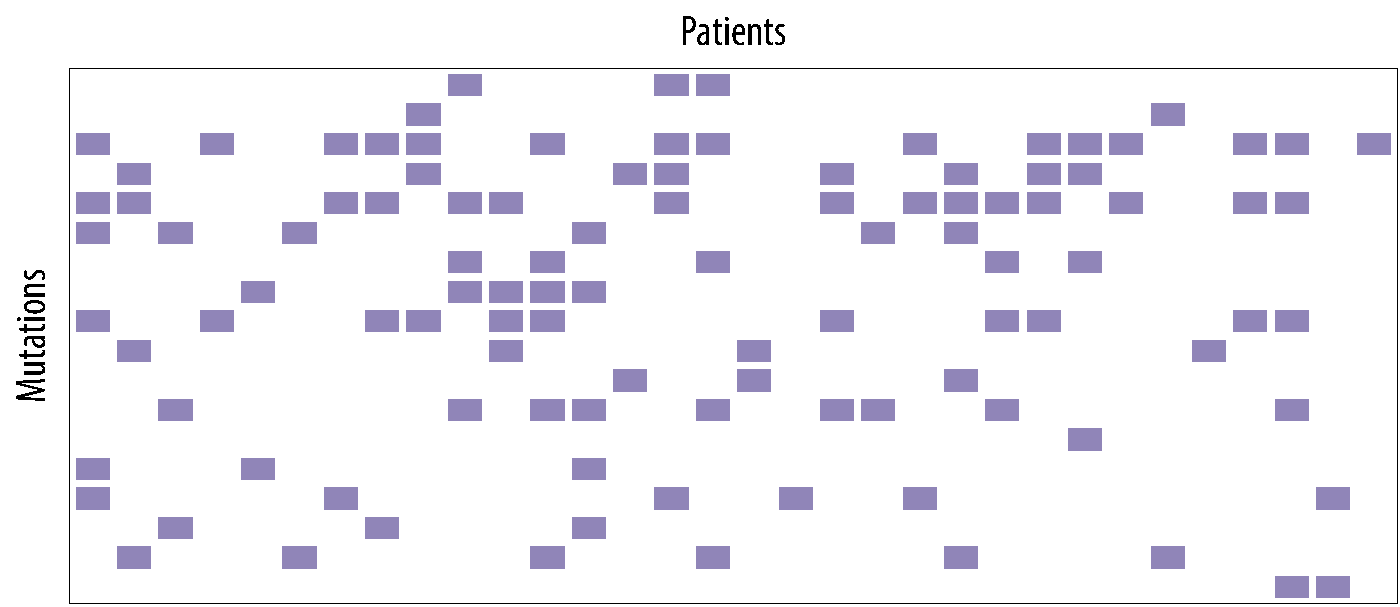
\includegraphics[width=0.95\textwidth]{figures/intro/example1.pdf}\\[1em]
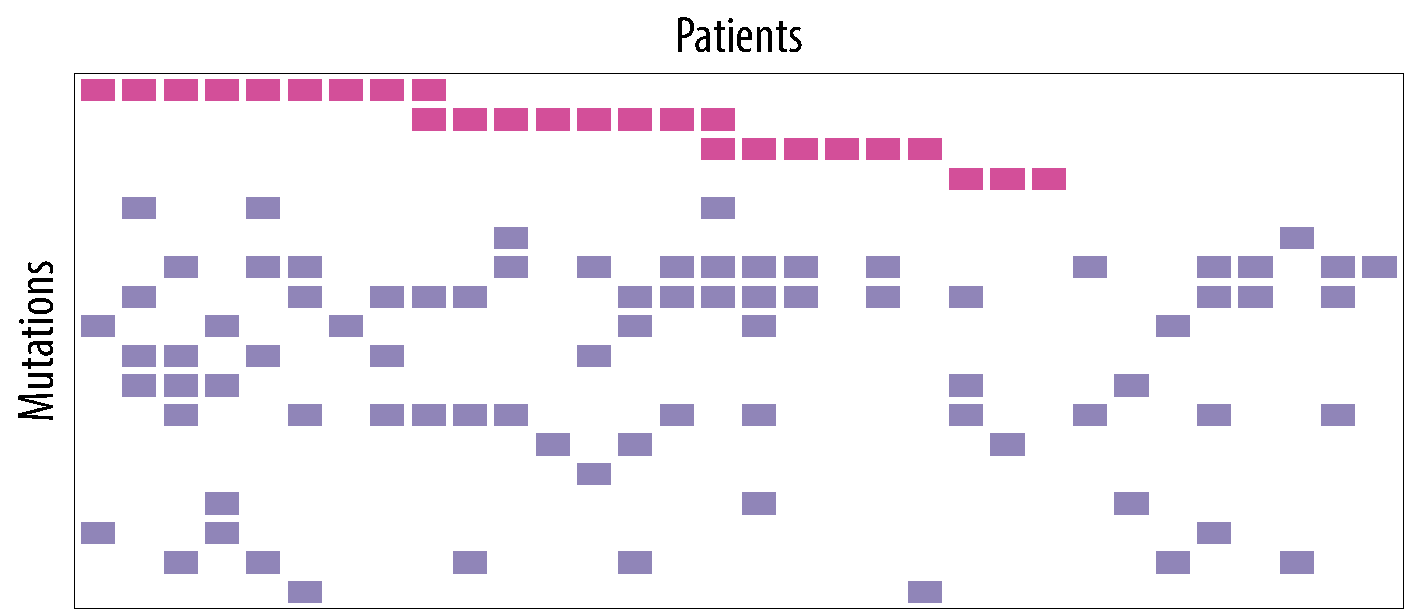
\includegraphics[width=0.95\textwidth]{figures/intro/example1_rep.pdf}\\[1em]
\caption{
(top) An example binary mutation matrix, in which each shaded entry $(i, j)$ indicates that mutation $i$ occured in patient $j$.
(bottom) The same matrix with permuted rows and columns to illustrate the mutual exclusivity between the first four mutations.
}
\label{fig:bamat}
\end{figure}

Many other practical machine learning problems are of similar nature, that is, like the problem described above, they consist in choosing one or more subsets out of a set of finite elements.
Examples include sensor placement \citep{krause06}, active learning \citep{golovin11}, influence maximization \citep{kempe03}, image segmentation \citep{jegelka11}, and document summarization \citep{lin11}.
While discrete optimization methods have been successful in many of these applications, it is often advantageous to go beyond optimization, and consider discrete probabilistic models.

The probabilistic nature of such models offers a way to deal with noisy data, and provides a flexible framework to robustly answer queries pertaining to the problem at hand.
Rather than obtaining a single optimum as the solution to our problem, we have a way to quantify our uncertainty about the most likely configurations, and make robust decisions based on computing various marginal and conditional probabilities of interest.
In addition, the use of probabilistic models suggests a principled approach for learning the potentially complex interactions present in the data, namely maximizing the likelihood of the model parameters.
Finally, constraining ourselves to specific model classes allows us to incorporate prior assumptions about the problem structure, and alleviate the scarce data issue.

\section{Probabilistic Submodular Models}
One one hand, past research on discrete probabilistic models has primarily focused on models defined by pairwise interactions, such as Markov random fields \citep{koller09}.
In many applications, however, it is of importance to directly capture higher-order dependencies between larger groups of variables.
For example, in our aforementioned application, being able to directly encode larger groups of mutually exclusive mutations provides a potentially sparser and easier to interpret representation, while at the same time it allows for a richer structure of interactions.

On the other hand, in the context of discrete optimization, there has been extensive research on submodular set functions.
Submodularity is a diminishing returns property that has been used to encode repulsiveness, diversity, or exclusivity.
Analogously, its counterpart, supermodularity, has been used to encode attractiveness, cooperation, or co-occurence.
Notably, there exist well-known efficient algorithms for both approximate submodular maximization as well as submodular minimization.

Merging these two directions naturally leads us to consider \emph{probabilistic submodular models} \citep{djolonga14,gotovos15}, a class of discrete probabilistic models defined by submodular (or supermodular) functions.
More concretely, given a ground set $V = \{1,\ldots n\}$, a probabilistic submodular model is a distribution over subsets of $V$ of the form
\begin{align*}
p(S; \btheta) = \frac{1}{Z(\btheta)} \exp\left( F(S; \btheta) \right),
\end{align*}
for all $S \subseteq V$, where $F$ is a submodular or supermodular function parameterized by $\btheta$, and $Z(\btheta)$ is the normalizer of the distribution.
Distributions of this form generalize some well-studied model classes, such as Ising models and determinantal point processes.

\section{Thesis Topic \& Contributions}
Both learning the model parameters $\btheta$ from data, as well as quantifying uncertainty and making decisions with the learned distribution, boil down to the fundamental task of probabilistic inference, that is, computing the normalizer $Z$ or various marginal probabilities of such distributions, a problem that is known to be computationally intractable in general.
The main topic of this thesis is to investigate the use of Markov chain Monte Carlo sampling as a means of performing approximate inference in probabilistic submodular models.

The primary contributions of this thesis can be summarized as follows.
\begin{itemize}[leftmargin=3.5em]
\item[\textsf{Chapter 3}] We analyze the Gibbs sampler in probabilistic submodular models, and prove sufficient theoretical conditions for polynomial-time, and fast---$\mathcal{O}(n\log n)$---mixing.
\item[\textsf{Chapter 4}] We propose a novel sampler that makes use of discrete semigradients to perform efficient global moves in the state space to avoid bottlenecks, thus leading to improved mixing compared to the Gibbs sampler.
\item[\textsf{Chapter 5}] We use sampling to learn probabilistic submodular models via approximate likelihood maximization, and apply this procedure to the problem of modeling interactions between genetic mutations in cancer patients.
Many of our results demonstrate considerable improvement over the state of the art.
\end{itemize}

\section{Collaborators}
The topic of sampling from probabilistic submodular models was conceived by my advisor, Prof. Andreas Krause, who has also contributed to most parts of this thesis by providing large amounts of input and feedback over the years.
Parts of the theoretical analysis in \chapref{ch:gibbs} and \chapref{ch:m3} were done in collaboration with Prof. Hamed Hassani.
The work of \chapref{ch:m3} was done under the guidance of Prof. Stefanie Jegelka, who also contributed to the theoretical analysis of this chapter.
Finally, regarding the application presented in \chapref{ch:genes}, I have had several fruitful discussions with Gideon Dresdner, Dr. Kjong Lehmann, and Prof. Gunnar Rätsch.